%# -*- coding: utf-8-unix -*-
%%==================================================
\chapter{计算机网络}
\label{chap1}
\begin{itemize}[noitemsep,topsep=0pt,parsep=0pt,partopsep=0pt]
	\item ...
\end{itemize}

\section{知识点和方法论}
\subsubsection{查看端口信息}
netstat -a // 显示所有的端口信息
\subsubsection{SYN攻击}
简单的说是三次握手环节, 攻击者发送SYN请求, 然后就消失了, 导致服务器上大量的资源尝试去进行SYN响应.

解决办法, 降低SYN timeout时间,使得主机尽快释放半连接的占用

\subsubsection{arp协议}
根据IP地址查询相应的以太网MAC地址

\subsubsection{DNS过程}
1. 先从DNS缓存中, 本地缓存或者路由器缓存中查找ip地址. DNS根服务器, .com服务器, .server.com 服务器 三级查找

\begin{figure}
	\centering
	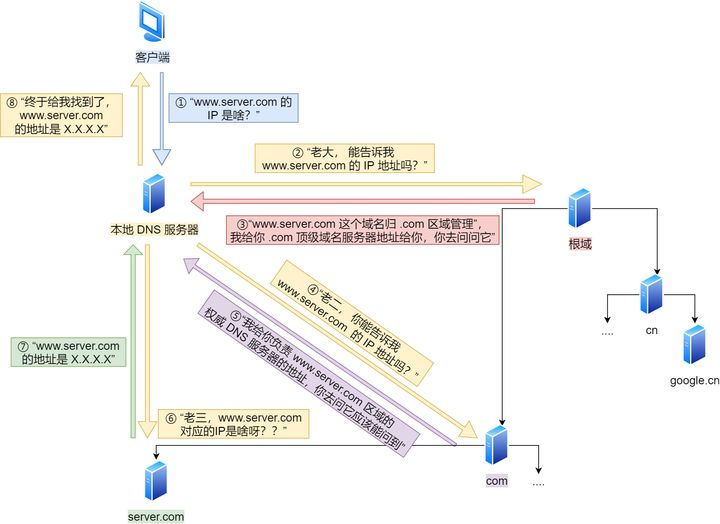
\includegraphics[width=0.7\linewidth]{figures/dns.jpg}
	\caption{dns}
	\label{fig:dns}
\end{figure}



\subsubsection{TCP如何保证可靠性}
1. 校验和: 通过添加16btye的校验和

2. 确认信号ACK与序列号
数据发送后, 对方回发送一个ack表示数据已经收到了 比如服务端发送了1-1000的数据, ack应答1001 表示前1000个数据已经送达了.

3. 超时重传: 报文发出后在一定时间内未收到接收方的应答, 发送方就会进行重发.

4. 连接管理机制: 三次握手和四次挥手

5. 流量控制: 接收端处理数据的速度是有限的,如果发送方发送数据的速度过快,导致接收端的缓冲区满,而发送方继续发送,就会造成丢包,继而引起丢包重传等一系列连锁反应。
因此TCP支持根据接收端的处理能力,来决定发送端的发送速度,这个机制叫做流量控制。
在TCP报文段首部中有一个16位窗口长度,当接收端接收到发送方的数据后,在应答报文ACK中就将自身缓冲区的剩余大小,放入16窗口大小中。这个大小随数据传输情况而变,窗口越大,网络吞吐量越高,而一旦接收方发现自身的缓冲区快满了,就将窗口设置为更小的值通知发送方。如果缓冲区满,就将窗口置为0,发送方收到后就不再发送数据,但是需要定期发送一个窗口探测数据段,使接收端把窗口大小告诉发送端。

6. 拥塞控制
然而如果网络非常拥堵,此时再发送数据就会加重网络负担,那么发送的数据段很可能超过了最大生存时间也没有到达接收方,就会产生丢包问题。
为此TCP引入慢启动机制,先发出少量数据,就像探路一样,先摸清当前的网络拥堵状态后,再决定按照多大的速度传送数据。
此处引入一个拥塞窗口:
发送开始时定义拥塞窗口大小为1;每次收到一个ACK应答,拥塞窗口加1;而在每次发送数据时,发送窗口取拥塞窗口与接送段接收窗口最小者。
慢启动:在启动初期以指数增长方式增长;设置一个慢启动的阈值,当以指数增长达到阈值时就停止指数增长,按照线性增长方式增加;线性增长达到网络拥塞时立即“乘法减小”,拥塞窗口置回1,进行新一轮的“慢启动”,同时新一轮的阈值变为原来的一半。慢启动, 拥塞避免, 快重传, 快恢复. \par

\subsubsection{TCP报文头部内容}
1. 源端口

2. 目的端口

3. 校验和

4. ACK标志位

5. FIN 标志位

6. 校验和

7. 序号seq和确认号ack


\subsubsection{TCP三次握手和四次挥手示意图}
\url{https://www.cnblogs.com/eat-too-much/p/14764778.html}
\url{https://www.cnblogs.com/eat-too-much/p/14765125.html}
\begin{figure}
	\centering
	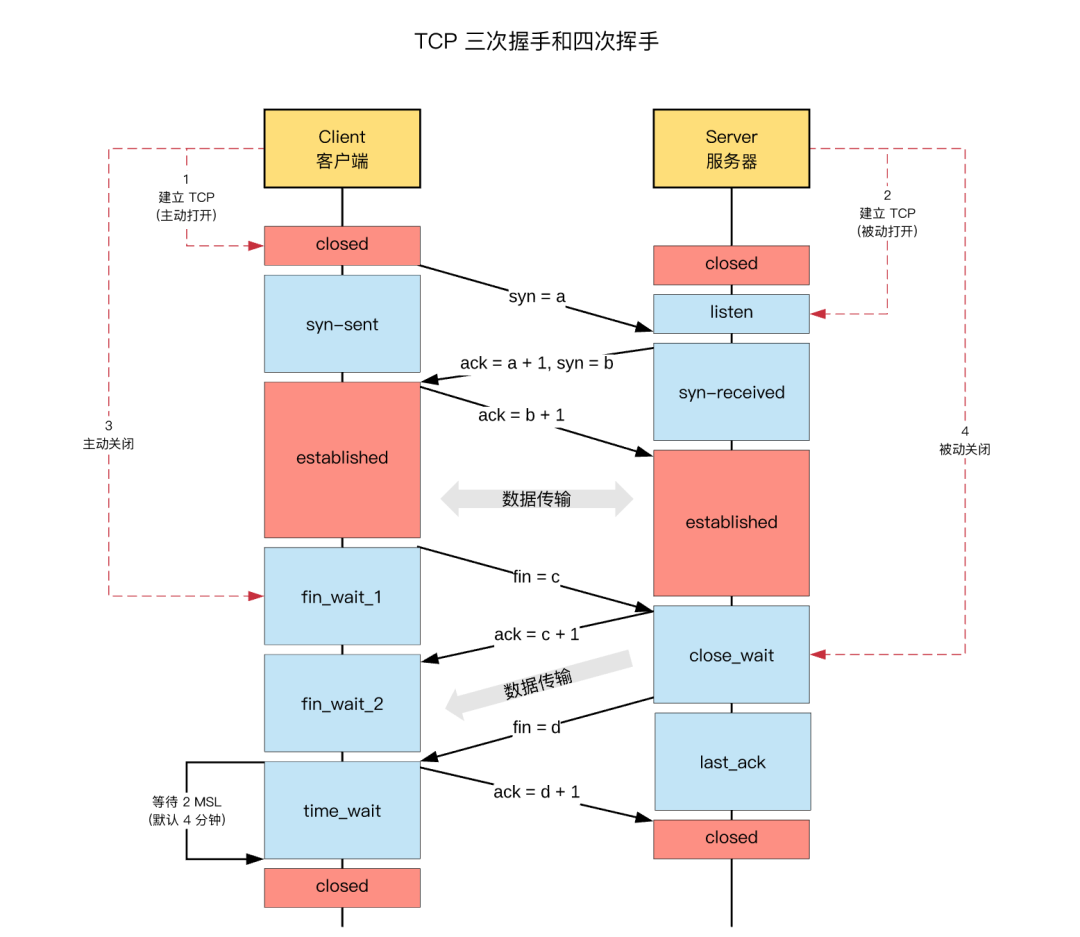
\includegraphics[width=0.7\linewidth]{figures/tcpconnectdis.png}
	\caption{tcpconnectdis}
	\label{fig:tcpconnectdis}
\end{figure}
\subsubsection{Time\_wait状态}
1. 一个TCP连接中, 主动关闭连接的一方发现的状态; 收到FIN命令, 进入TIME\_WAIT状态, 并返回ACK命令

2. 保持两个MSL时间, 即4分钟; (MSL为2分钟)

如果在高并发场景下, 出现了大量的tcpTimewait状态. 如何解决? 因为tcp头中有16bit表示端口号. 如果65536个端口号因为timewait状态被占用, 系统就无法给出可用的服务.

缩减time\_wait时间, 设置为1msl.

服务端中可以设置为不必等待2MSL时间结束, 即可使用被占用的端口
\subsubsection{SYN-RCVD状态}
简单来说, 就是三次建立连接的时候, 对方没有把最后一次ack发送回来的时候的状态. 可能是别人攻击服务器产生的. \par

开启cookie检查校验连接的合法性

net.ipv4.tcp\_syncookies = 1
\begin{figure}
	\centering
	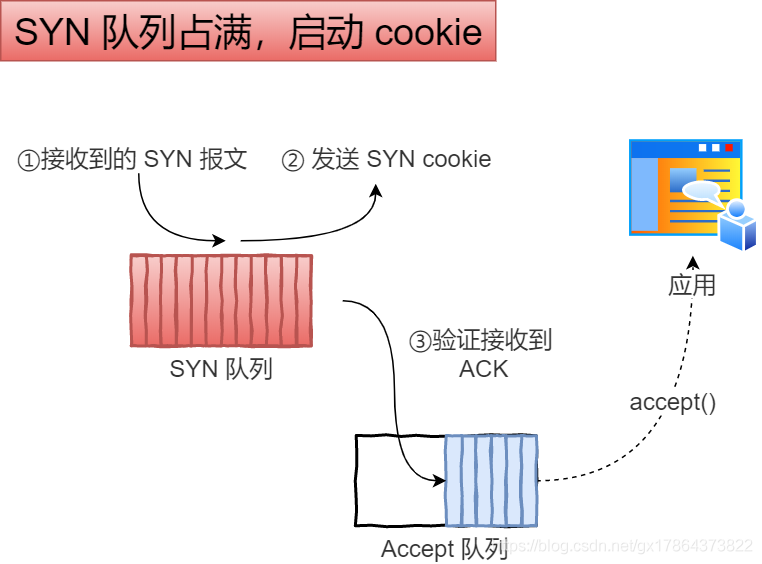
\includegraphics[width=0.7\linewidth]{figures/tcpsynrcvd.png}
	\caption{tcpsynrcvd}
	\label{fig:tcpsynrcvd}
\end{figure}
\subsubsection{TCP四个计时器}
1、重传计时器

一段时间没有接收到应答,则开始重新传输数据, 约60s

2. FIN 时间等待计时器

时间等待计时器是在连接终止期间使用的 。当TCP关闭一个连接时,它并不认为这个连接马上就真正地关闭了。在时间等待期间中,连接还处于一种中间过渡状态。这就可以使重复的FIN报文段(如果有的话)可以到达目的站因而可将其丢弃。这个计时器的值 通常设置为一个报文段的寿命期待值的两倍 。

3. 保活计时器

保活计时器 通常设置为2小时 。若服务器过了2小时还没有收到客户的信息,它就发送探测报文段。若发送了10个探测报文段(每一个相隔75秒)还没有响应,就假定客户出了故障,因而就终止该连接。

4、坚持计时器

当发送TCP收到一个窗口大小为零的确认时,就启动坚持计时器 。 当坚持计时器期限到时,发送TCP就发送一个特殊的报文段, 叫做 探测报文段 。这个报文段只有一个字节的数据。它有一个序号,但它的序号永远不需要确认;甚至在计算对其他部分的数据的确认时该序号也被忽略。探测报文段提醒对端:确认已丢失,必须重传。
\subsubsection{TCP流量控制}
简单来说, 接收端通过返回一个win参数告诉发送端还能发送多少. 如果不能发送了的话, 开启坚持定时器, 去发送试探帧, 如果又可以发送了的话,继续发送. \par
新一代算法采用google的BBR算法.

TCP BBR \textbf{不再使用丢包作为拥塞的信号},也不使用 “加性增,乘性减” 来维护发送窗口大小,而是分别估计极大带宽和极小延迟,把它们的乘积作为发送窗口大小。
\begin{figure}
	\centering
	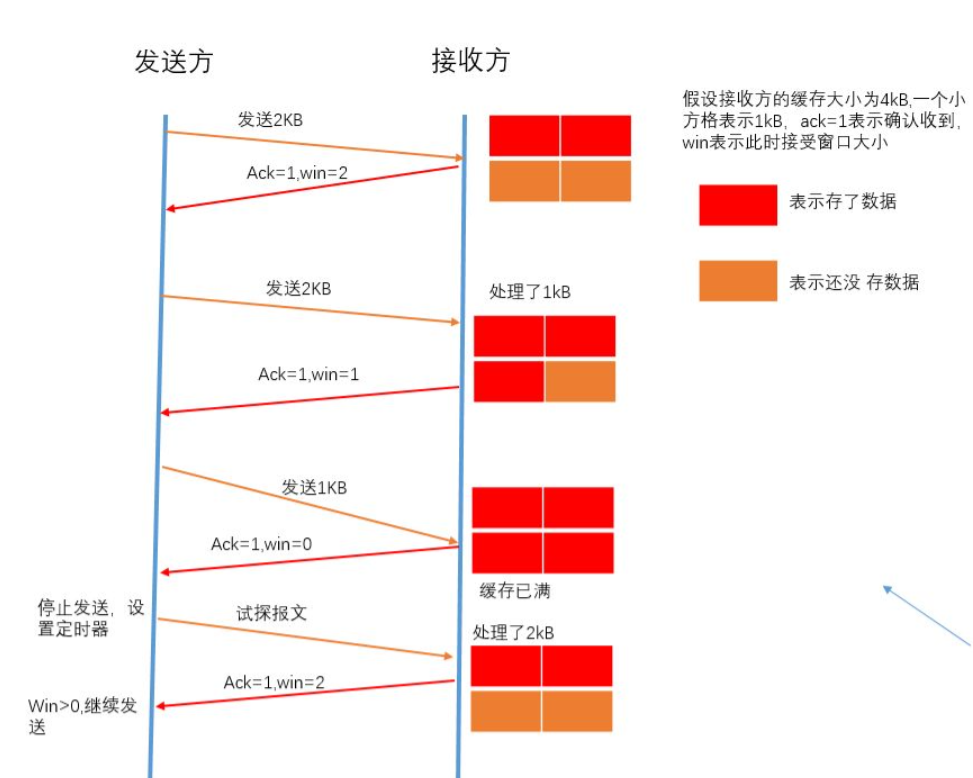
\includegraphics[width=0.7\linewidth]{figures/liuliangkongzhi.png}
	\caption{liuliangkongzhi}
	\label{fig:liuliangkongzhi}
\end{figure}
\subsubsection{HTTPS访问过程, SSL 握手的过程}
证书主要作用是在SSL握手中,我们来看一下SSL的握手过程

1. 客户端提交https请求

2. 服务器响应客户,并把证书公钥发给客户端

3. 客户端验证证书公钥的有效性

4. 有效后,会生成一个会话密钥

5. 用证书公钥加密这个会话密钥后,发送给服务器

6. 服务器收到公钥加密的会话密钥后,用私钥解密,回去会话密钥

7. 客户端与服务器双方利用这个会话密钥加密要传输的数据进行通信

\begin{figure}
	\centering
	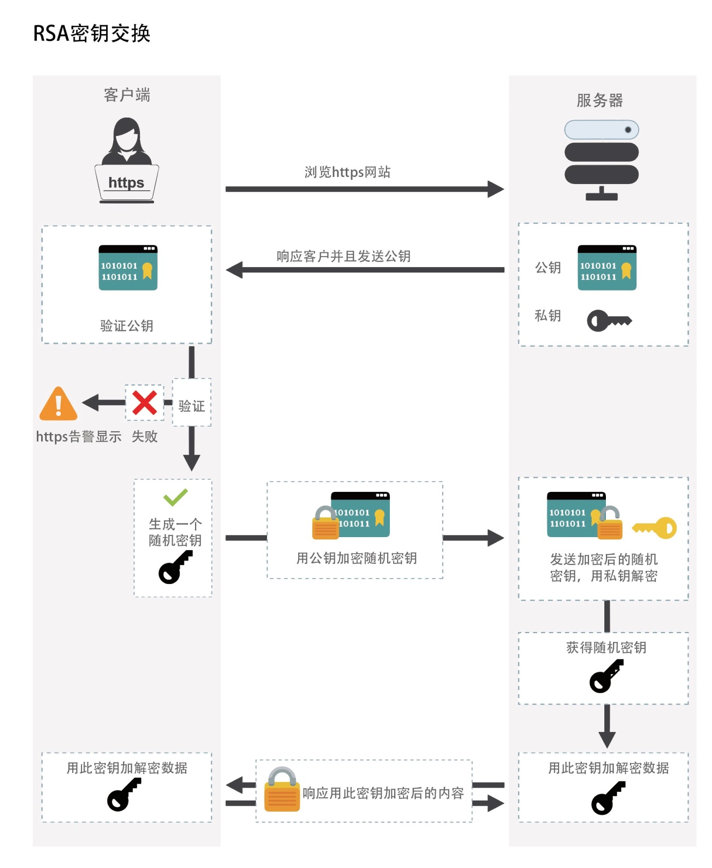
\includegraphics[width=0.7\linewidth]{figures/https.png}
	\caption{https}
	\label{fig:https}
\end{figure}

\subsubsection{计算机网络分层}
计算机网络OSI模型是七层, 如果是TCP/IP则是四层
\begin{figure}
	\centering
	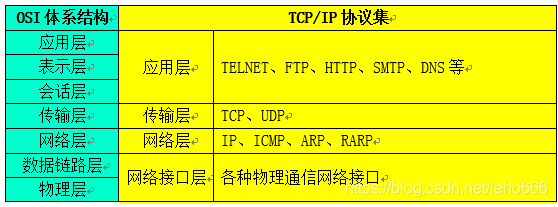
\includegraphics[width=0.7\linewidth]{figures/TCP_IP_OSI.png}
	\caption{TCP\_IP\_OSI}
	\label{fig:TCP_IP_OSI}
\end{figure}
\begin{figure}
	\centering
	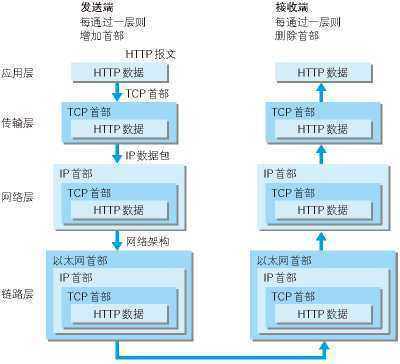
\includegraphics[width=0.7\linewidth]{figures/osi.jpg}
	\caption{osi}
	\label{fig:osi}
\end{figure}
\subsubsection{TCP和UDP区别?}
\par
UDP: 面向报文, 支持1对1, 1对多, 多对1的交互通信
\par
TCP: 面向连接, 提供可靠交付, 有流量控制, 拥塞控制, 提供全双工通信, 面向字节流. TCP是点对点的.
\subsubsection{TCP三次握手相关问题}
为什么三次握手而不是两次握手: 主要是为了防止已失效的链接请求报文段突然又传送到了B, 因而产生错误. 如果只要两次握手就建立连接, 那么如果A第一次请求丢失了, A 又发送了一次请求, 但是这一次传输结束了, A上一次丢失的请求再次被传送到了B, 如果建立了连接, 但是A现在一直不回应B, 导致B浪费了资源.
\subsubsection{TCP四次挥手问题}
关闭连接的时候, 当Server端收到FIN报文时候, 很可能并不会立即关闭SOCKET, 所以只能先回复一个ACK报文, 告诉Client端, 你发送的FIN我收到了, 只有等我Server端所有的报文都发送完了, 我才能发送FIN报文. 不能一起发送, 所以需要四步挥手.
\subsubsection{TCP协议-如何保证传输的可靠性}
\textbf{超时重传:} 简单理解就是发送在发送完数据后等待一个时间, 时间到大没有接收到ACK报文, 那么对刚才发送的数据进行重新发送
\par
\textbf{连接管理:} 使用三次握手和四次挥手
\par
\textbf{流量控制:} TCP根据接收端对数据的处理能力, 决定发送端的发送速度, 这个机制就是流量控制. TCP协议的包头信息当中, 有一个16位字段的窗口大小, 发送方更具ACK报文里的窗口大小的值的改变自己的发送数据
\par
\textbf{拥塞控制:} 慢开始, 拥塞避免, 快重传, 快恢复.
\par
慢开始算法的思路就是, 不要一开始就发送大量的数据, 先探测一下网络的拥塞程度, 也就是说由小到大主键增加拥塞窗口的大小.
\par
拥塞避免算法让拥塞窗口缓慢增长, 即每经过一个往返时间RTT就把发送方的拥塞窗口cwnd加1, 而不是加倍. 这样拥塞窗口按线性归路缓慢增长.
\par
快重传和快恢复: 发送方只要一脸收到三个重复确认就引动立即重传对方尚未收到的报文段, 而不必继续等待设置的重传计时器时间到器.
\begin{figure}
	\centering
	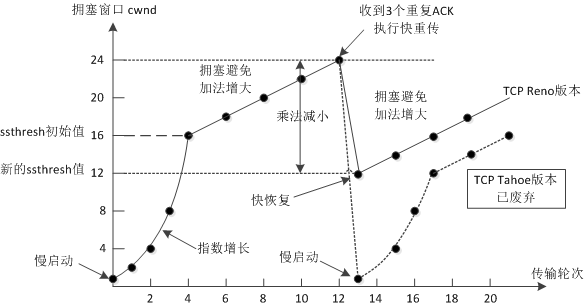
\includegraphics[width=0.7\linewidth]{figures/tcp.png}
	\caption{tcp}
	\label{fig:tcp}
\end{figure}
\subsubsection{Cookie作用, 安全性问题和Session的比较}
(1) Cookie是服务器发送到用户浏览器并保存在本地的一小块数据,  他会在浏览器之后向统一服务器再次发送请求时被携带上.
\par
(2) Session 存储在服务器端. 使用Session维护用户登录状态的过程如下: (需要cookie作为传输机制)
用户进行登陆是, 用户提交包含用户名和密码的表单, 放入HTTP请求报文中;
服务器校验该用户名和密码, 如果正确则把用户信息存储到Redis中, 他在Redis中的key成为SessionId.
\par
服务器返回的响应报文Set-Cookie首部字段包含了这个SessionID, 客户端收到响应报文之后将该Cookie值存入浏览器中.客户端之后对同一个服务器进行请求时会包含该Cookie值, 服务器收到之后提取出SessionID, 从Redis中取出用户信息, 继续之前的业务操作.
\par
session 的运行依赖 session id, 而 session id 是存在 cookie 中的, 也就是,如果浏览器禁用了 cookie, 同时 session 也会失效(但是可以通过其它方式实现, 比如在 url 中传递 session\_id)
\par
cookie存在大小限制, 单个不超过4k, 浏览器中Cookie个数也有限制.
Session没有大小限制, 是和服务器内存有关的.
\subsubsection{HTTP1.1 和 HTTP1.0的比较}
HTTP1.1 默认长链接, 长连接只需要建立一次TCP连接, 进行多次HTTP通信.

纯文本协议


HTTP1.0 默认短连接, 每进行一次HTTP通信就要新建一个TCP连接.
\subsubsection{HTTP2.0 和 HTTP1.1的比较}
2.0 特点

多路复用: 所有HTTP2.0通信都在一个TCP链接上完成,这个链接可以承载任意流量的双向数据流。

二进制分帧: + 头部压缩

服务器推送:服务器除了最初请求的响应外,服务器还可以额外向客户端推送资源,而无需客户端明确的需求。

这种方式如何防止接受混乱呢?

在HTTP2.0上,客户端和服务器可以把HTTP 消息分解为互不依赖的帧,然后乱序发送,最后再在另一端把它们重新组合起来。注意,同一链接上有多个不同方向的数据流在传输。客户端可以一边乱序发送stream,也可以一边接收者服务器的响应,而服务器那端同理。(简单来说就是, 根据请求头来组件一个整个数据)

也会遇到队头阻塞, TCP层面上.

1.1

对头阻塞: 如果4丢了, 那么收到的5-8都没用.
有非管道化和管道化,两种方式。

非管道化,完全串行执行,请求->响应->请求->响应...,后一个请求必须在前一个响应之后发送。

管道化,请求可以并行发出,但是响应必须串行返回。后一个响应必须在前一个响应之后。原因是,没有序号标明顺序,只能串行接收。

管道化请求的致命弱点:

1. 会造成队头阻塞,前一个响应未及时返回,后面的响应被阻塞
2. 请求必须是幂等请求,不能修改资源。因为,意外中断时候,客户端需要把未收到响应的请求重发,非幂等请求,会造成资源破坏。

由于这个原因,目前大部分浏览器和Web服务器,都关闭了管道化,采用非管道化模式。

无论是非管道化还是管道化,都会造成队头阻塞(请求阻塞)。

\subsubsection{HTTP3.0}

QUIC协议:

前项纠错机制: 称为向前纠错(Foward Error Connec,FEC),每个数据包除了它本身的内容之外还包括了其他数据包的数据,因此少量的丢包可以通过其他包的冗余数据直接组装而无需重传。

基于UDP的协议.

自定义连接机制:

TCP基于四元数,IP, 目标IP, 目标port, 自己的port. 一旦一个元素发生变化,就会重新建立连接.
但是, QUIC使用一个64位随机数来确定这个连接. 三次握手的时间减少. 也减少二路TLS的时间.




\subsubsection{HTTPS加密}
使用SSL连接. HTTPS采用混合加密算法, 使用非对称加密和对称加密, 非对称加密用于传输对称秘钥来保证传输过程的安全性, 之后使用对称秘钥加密进行通信来保证通信过程的效率.
\par
HTTPS加密过程:
\begin{enumerate}
	\item 客户使用HTTPS的URL访问web服务器, 要求与Web服务器建立SSL链接.
	\item Web服务器收到客户端请求后, 会将网站的证书信息(证书中包含公钥)传送一份给客户端.
	\item 客户端的浏览器与web服务器开始写上SSL链接的安全登记, 也就是信息加密登记.
	\item 客户端的浏览器更具双方同意的安全登记, 建立会话秘钥, 然后利用网站的公钥将会话秘钥加密, 并传送给网站
	\item Web服务器利用自己的私钥解密出会话秘钥.
	\item Web服务器利用会话秘钥加密与客户端之间的通信.
\end{enumerate}
\par
缺点: 因为需要进行加密解密等过程, 因此速度会更慢, 需要支付证书授权的高额费用.
\subsubsection{输入网址发生的事情}
\begin{enumerate}
	\item 浏览器查找该域名的IP地址
	\item 浏览器更具解析得到的IP地址向web服务器发送一个HTTP请求.
	\item 服务器收到请求并进行处理
	\item 服务器返回一个响应.
	\item 浏览器对该响应进行解码, 渲染显示.
	\item 页面显示完成后, 浏览器发送异步请求.
\end{enumerate}